\documentclass[12pt]{article}

\usepackage[margin=0.8 in]{geometry}
\usepackage{amsmath}
\usepackage{amssymb}
\usepackage{mathtools}
\usepackage{enumerate}
\usepackage{verbatim}
\usepackage{amsthm}
\usepackage{hyperref}
\usepackage{caption}

\title{Parametrizing surfaces}
%\content{}



\let \proj \undefined
\newcommand{\p}{\partial}
\newcommand{\R}{ \mathbb{R}}

\DeclareMathOperator{\proj}{proj}
\newcommand{\sS}{\mathscr{S}}
\DeclareMathOperator{\comp}{comp}
\newcommand{\A}{\mathcal{A}}
\newcommand{\D}{\mathcal{D}}
\newcommand{\e}{\epsilon}
\newcommand{\et}{\tilde{\e}}
\newcommand{\vr}{\vec{r}{}}
\newcommand{\vF}{\vec{F}}
\newcommand{\triple}{\iiint_E f(x,y,z)dV}
\renewcommand{\lg}{\langle}
\newcommand{\rg}{\rangle}
\newcommand{\Q}{\frac{\p Q}{\p x}}
\renewcommand{\P}{\frac{\p P}{\p y}}
\let\implies\Rightarrow
\newcommand{\n}{\nabla}
\newcommand{\Fline}{\vF\cdot d\vr}
\newcommand{\vi}{\vec{i}}
\newcommand{\vj}{\vec{j}}
\newcommand{\vk}{\vec{k}}
\DeclareMathOperator{\curl}{curl}
%\newcommand{\n}{\nabla}




\newenvironment{solution}
  {\begin{proof}[Solution]}
  {\end{proof}
  
  }
\newtheorem{example}{Example}
\newtheorem{exercise}{Exercise}
\newtheorem{theorem}{Theorem}
\newtheorem{definition}{Definition}


\begin{document}
\maketitle
\begin{enumerate}
\item \textbf{Ellipsoids:} The ellipsoid $$\dfrac{x^2}{a^2}+\dfrac{y^2}{b^2}+\dfrac{z^2}{c^2}=1$$ can be parametrized by setting $$\vr(u,v)=\lg a\sin(u)\cos(v),b\sin(u)\sin(v),c\cos(u)\rg \text{ for }(u,v)\in [0,\pi]\times[0,2\pi].$$

As a special case, the \textbf{sphere} $x^2+y^2+z^2=r^2$ can be parametrized as $$\vr(u,v)=\lg r\sin(u)\cos(v),r\sin(u)\sin(v),r\cos(u)\rg \text{ for }(u,v)\in [0,\pi]\times[0,2\pi].$$

\begin{figure}[h]
\centering
\parbox{5cm}{
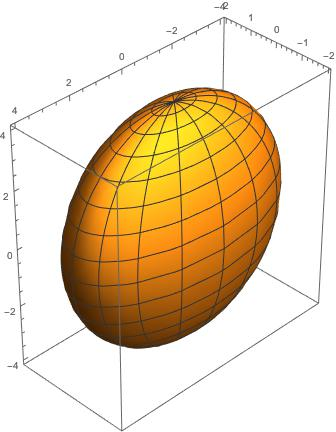
\includegraphics[width=5cm]{ellipsoid.jpeg}
\caption{The ellipsoid  $\dfrac{x^2}{4}+\dfrac{y^2}{16}+\dfrac{z^2}{16}=1$}
\label{}}
\qquad
\begin{minipage}{5cm}
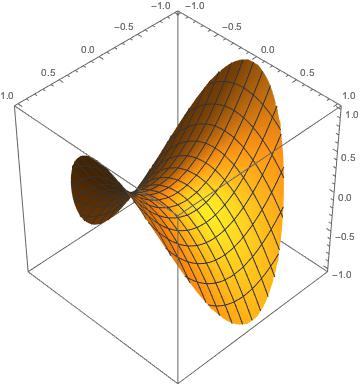
\includegraphics[width=5cm]{saddle.jpeg}
\caption{The graph of $f(x,y)=x^2-y^2$, for $(x,y)$ in the unit disk.}
\label{fig:2figsB}
\end{minipage}
\end{figure}



\item \textbf{Graphs:} When our surface is the graph of a function $f(x,y)$, where $(x,y)\in D$, we can let $x=u$, $y=v$  and $z=f(u,v)$, that is, $$\vr(u,v)=\lg u,v, f(u,v)\rg\text{ for }(u,v)\in D.$$


\item\textbf{Cylinders:} (in a broad sense, surfaces described by an equation that only involves 2 variables, e.g. $x^2+\dfrac{z^2}{4}=1$.) We look at the equation of the cylinder and parametrize as if it were a plane curve, with respect to $u$. Then set the third variable to be $v$.

In this example, we would write $x=\cos(u)$, $z=2\sin(u)$, $u\in [0,2\pi]$ and $y=v$, $v\in \R$. 


\item \textbf{Surfaces of Revolution:} Say that we'd like to parametrize the surface obtained by revolving the graph of $z=f(y)$, $y\in [a,b]$ around the $y$ axis. Then we can set $y=v$ and therefore, since for each $v$ we have a circle of radius $f(v)$ on the plane $y=v$, $$\vr(u,v)=\lg f(v)\cos(u),v,f(v)\sin(u)\rg, (u,v)\in[0,2\pi]\times [a,b].$$ We work similarly if we need to revolve about another axis.
\begin{figure}[h]
\centering
\parbox{5cm}{
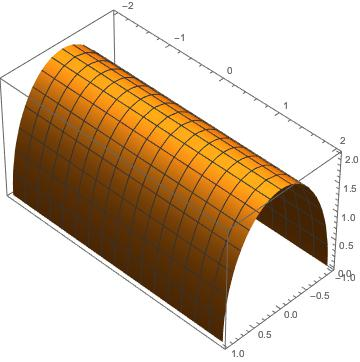
\includegraphics[width=5cm]{cylinder.jpeg}
\caption{The cylinder $x^2+\frac{z^2}{4}=1$, $z\geq 0$ parametrized as $x=\cos(u), y=v, z=2\sin(u)$, $u\in [0,\pi]$, $v\in\R$. }
\label{fig3}}
\qquad
\begin{minipage}{5cm}
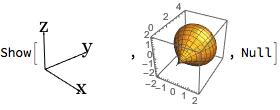
\includegraphics[width=5cm]{onion.jpeg}
\caption{Revolving the curve $z=1+\sin(y+\frac{3\pi}{2})$ around the $y$ axis, as $x=( \sin \left(v+\frac{3 \pi }{2})+1\right)\cos (u),$ $y=v$ and $z=$ \\$(\sin \left(v+\frac{3 \pi }{2})+1\right)\sin (u)$.}
\label{fig4}
\end{minipage}
\end{figure}

\item \textbf{Tori:} A torus (bagel) about the $z$ axis can be parametrized as 
$$\vr(u,v)=\lg (a+b\cos(v))\cos(u),(a+b\cos(v))\sin(u),b\sin(v)\rg, \text{ for }(u,v)\in [0,2\pi]\times[0,2\pi],$$ where $0<b<a$.
\begin{figure}[h]
\begin{center}
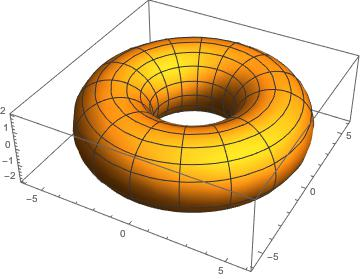
\includegraphics[scale=.3]{torus.jpeg}
\caption{A torus with parametrization $x=(4+2\cos(v))\cos(u),$ $y=(4+2\cos(v))\sin(u),$ $z=2\sin(v),$ for $(u,v)\in [0,2\pi]\times[0,2\pi].$}
\end{center}
\end{figure}
\end{enumerate}
\end{document}

